\appendix
\section*{Anhang}
\markboth{Anhang}{}
\addcontentsline{toc}{section}{Anhang}
\renewcommand{\thesubsection}{\Alph{subsection}}

\subsection{E-Mail von Carter Zenke über CS50}\label{appendix:carter-zenke}
\begin{lstlisting}[style=Bash]
Von: Carter Zenke <carter@cs50.harvard.edu>
Antworten an: "carter@cs50.harvard.edu" <carter@cs50.harvard.edu>
Datum: Samstag, 6. November 2021 um 01:26
An: Andreas Huber <andreas.huber@st.oth-regensburg.de>
Betreff: Re: [EXT] Re: Bachelor Thesis: Automated Code Review
 
Hi Andreas,
 
Unfortunately I don't think we're currently at a point where submit50, and
especially submit50.cs50.io, could be open source and public. I would hesitate
to give a timeline for rebuilding submit50, but would be happy for you to check
back in January!
 
All my best,
Carter
\end{lstlisting}

\newpage

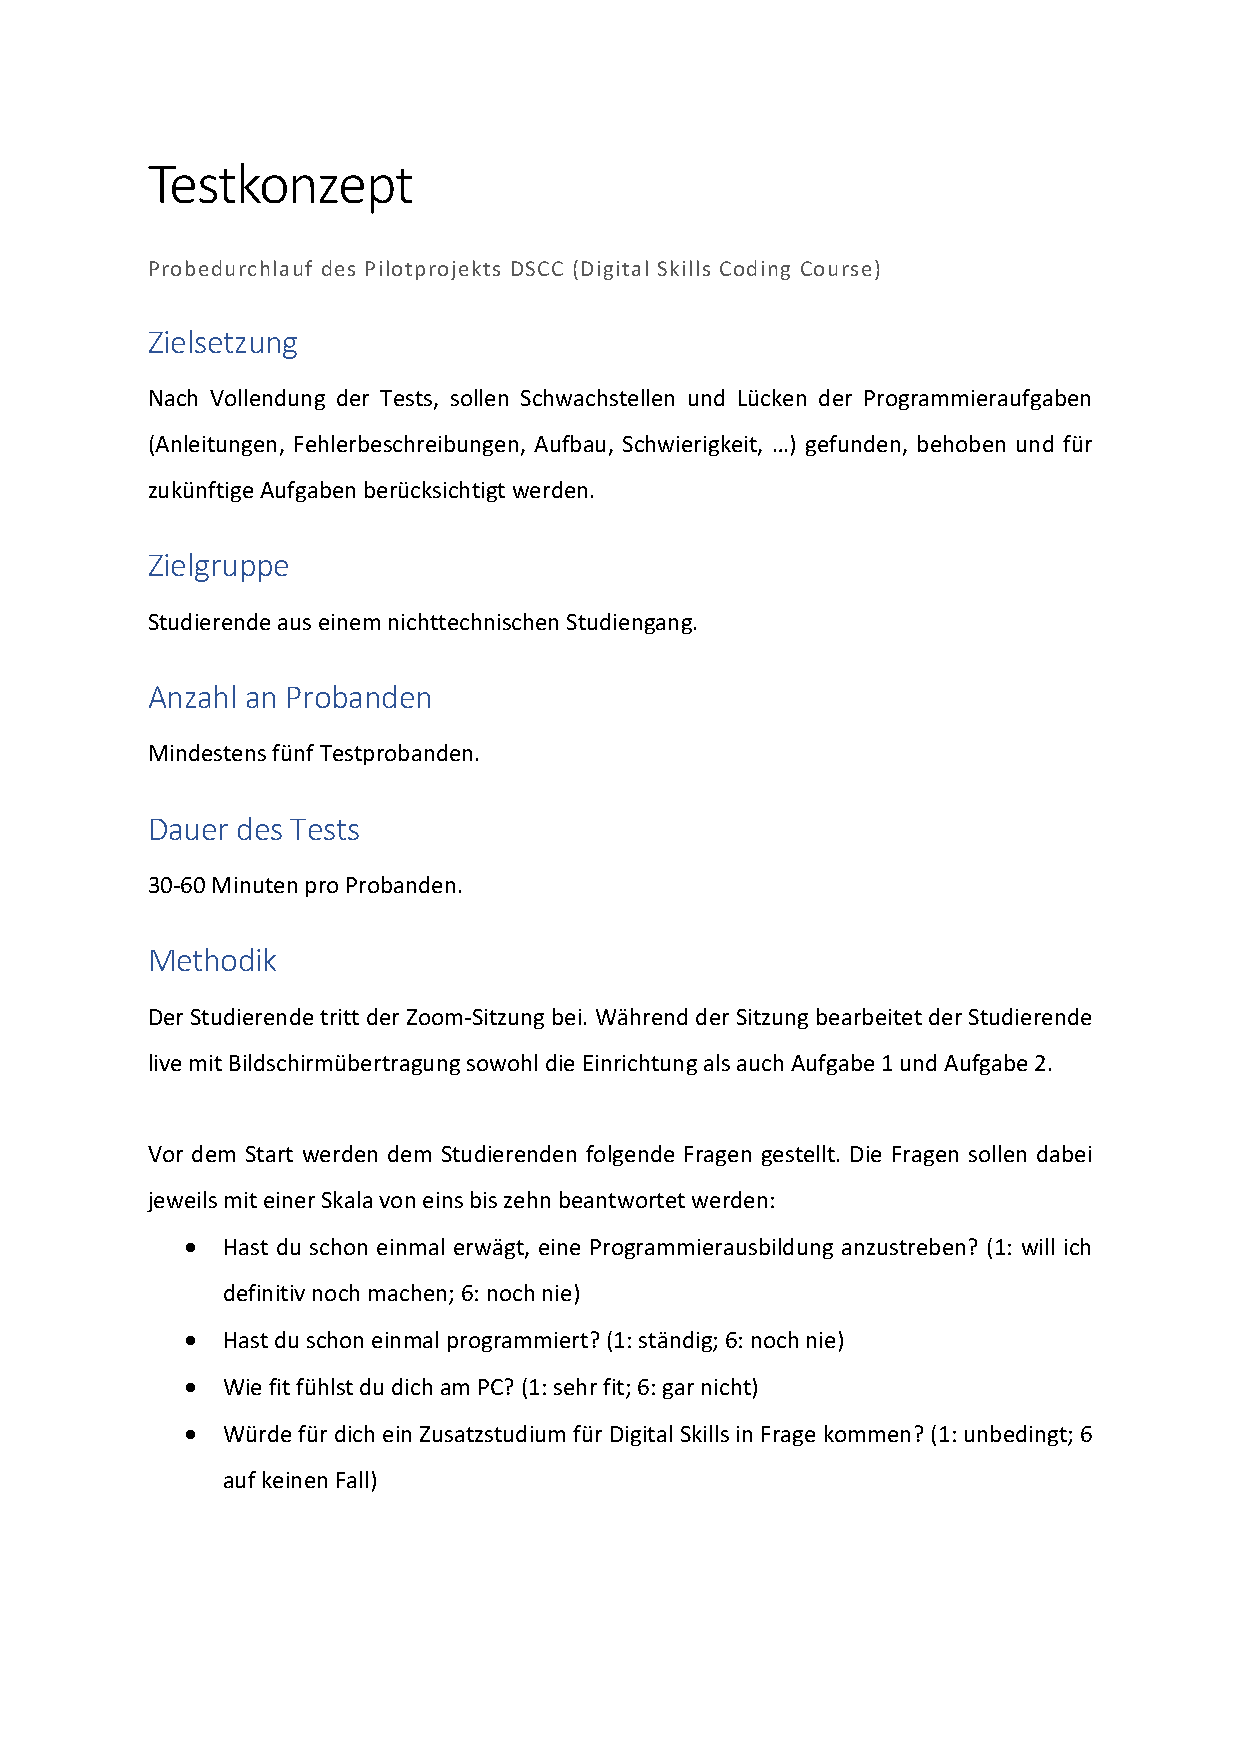
\includepdf[
    clip=0mm 0mm 0mm 0mm,
    trim=10mm 20mm 10mm 5mm,
    pages=1,
    frame,
    scale=.75,
    pagecommand=\subsection{Testkonzept Studie}\label{appendix:testkonzept}
 ]{assets/pdf/digital_skills_programmierkurs_testkonzept.pdf}
\includepdf[
    clip=0mm 0mm 0mm 0mm,
    trim=10mm 20mm 10mm 5mm,
    pages=2,
    frame,
    scale=.75,
    pagecommand={}
 ]{assets/pdf/digital_skills_programmierkurs_testkonzept.pdf}

 
\includepdf[
    clip=0mm 0mm 0mm 0mm,
    trim=10mm 20mm 10mm 5mm,
    pages=1,
    scale=.67,
    pagecommand=\subsection{Digital Skills Coding Course: Infodokument}\label{appendix:dscc-info}
 ]{assets/pdf/ds_zusammenfassung.pdf}

\newpage

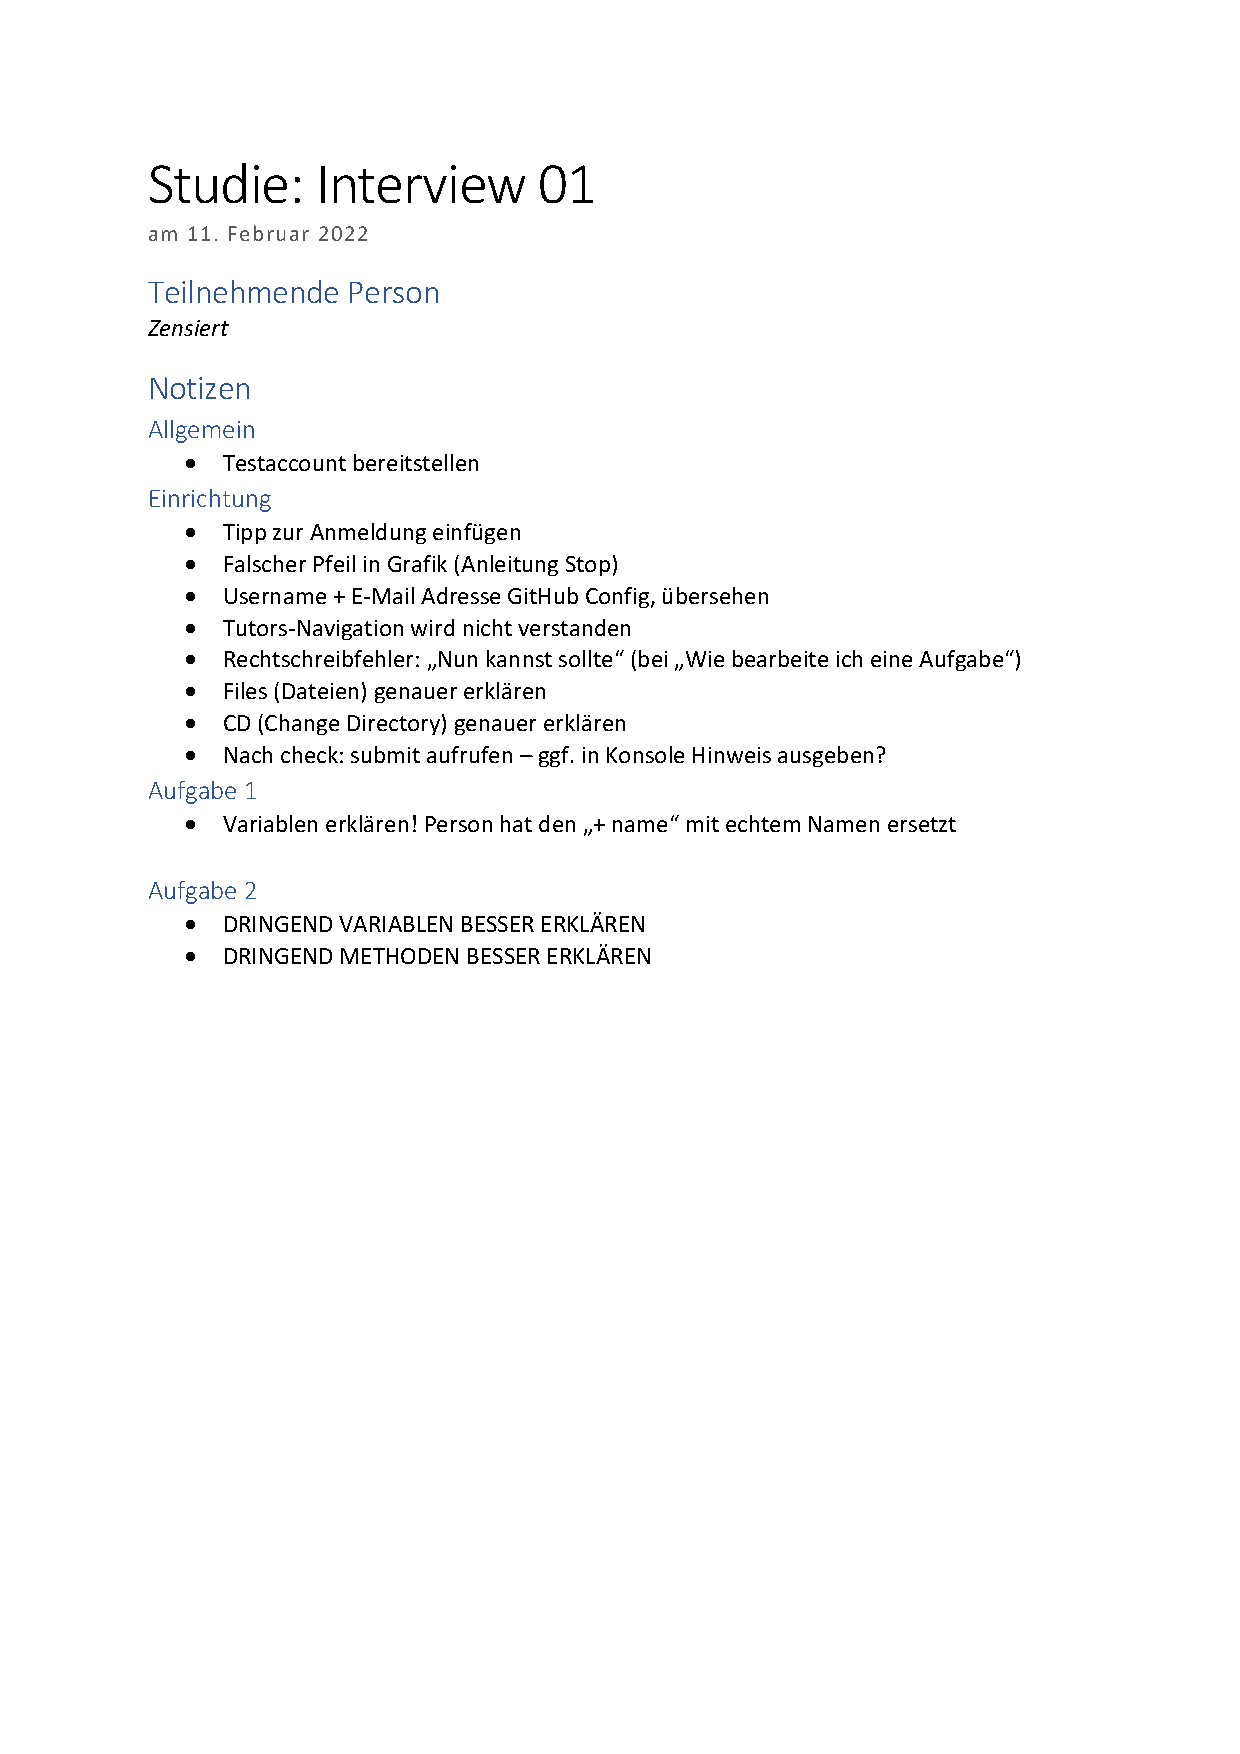
\includepdf[
    clip=0mm 0mm 0mm 0mm,
    trim=10mm 20mm 10mm 5mm,
    pages=1,
    frame,
    scale=.75,
    pagecommand=\subsection{Feldstudie: Beobachternotizen}\label{appendix:feldstudie-notizen}
 ]{assets/pdf/studienergebnisse.pdf}

 \includepdf[
    clip=0mm 0mm 0mm 0mm,
    trim=10mm 20mm 10mm 5mm,
    pages=2-,
    frame,
    scale=.75,
    pagecommand={}
 ]{assets/pdf/studienergebnisse.pdf}